\documentclass[12pt]{article}
\usepackage[margin=1in]{geometry}
\usepackage[T1]{fontenc}
\usepackage{lmodern}
\usepackage{microtype}
\usepackage{parskip}
\usepackage{xcolor}
\usepackage{listings}
\usepackage{graphicx}
\usepackage{float}
\usepackage{hyperref}
\usepackage{fancyhdr}

\hypersetup{
  pdftitle={DATA 200: Python Learning Log: Fictional Sample Entries},
  pdfauthor={Jason E. Czak},
  colorlinks=true,
  urlcolor=blue!60!black
}

\definecolor{codegreen}{RGB}{0,100,0}
\definecolor{codeblue}{RGB}{0,55,140}
\definecolor{codepurple}{RGB}{110,30,120}
\definecolor{lightgray}{RGB}{247,247,247}

\lstdefinestyle{pythonstyle}{
  language=Python,
  backgroundcolor=\color{lightgray},
  basicstyle=\ttfamily\small,
  keywordstyle=\color{codeblue}\bfseries,
  commentstyle=\color{codegreen},
  stringstyle=\color{codepurple},
  numbers=left,
  numberstyle=\tiny,
  numbersep=8pt,
  frame=single,
  breaklines=true,
  showstringspaces=false,
  columns=fullflexible,
  keepspaces=true
}
\lstset{style=pythonstyle}

\setlength{\headheight}{15pt}
\pagestyle{fancy}
\fancyhf{}
\lhead{Fictional Sample Python Learning Log}
\rhead{Week 1}
\cfoot{\thepage}

\newcommand{\entrydetails}[4]{%
\begin{description}
  \item[Time spent:] #1
  \item[Learning focus:] #2
  \item[Resources used:] #3
  \item[Python file:] \texttt{#4}
\end{description}}

% The programs live in ../src/sample_entries; a copy of this file sitting next to them also works.
\newcommand{\samplecode}[2]{%
  \IfFileExists{../src/sample_entries/#1}%
    {\lstinputlisting[caption={#2}]{../src/sample_entries/#1}}%
    {\lstinputlisting[caption={#2}]{#1}}}

% Every run screenshot in this fictional sample is a placeholder.
\newcommand{\screenshotplaceholder}[1]{%
  \begin{figure}[H]
    \centering
    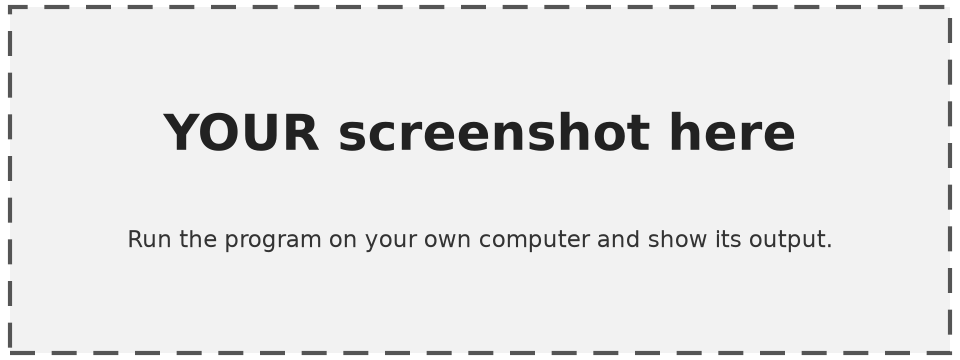
\includegraphics[width=0.7\textwidth]{screenshot-placeholder.png}
    \caption{#1 In your own log, this is a screenshot of your program running on your own computer.}
  \end{figure}}

\begin{document}

\begin{center}
{\LARGE\bfseries DATA 200: Python Learning Log}\par
\vspace{0.5em}
{\large Fictional Sample Entries: Week 1 Completed Example}\par
\end{center}

\textbf{Instructor note.} These entries are fictional models showing the expected level of detail. Students may document relevant homework, guided examples, or class exercises when those activities genuinely contributed to their Python learning. Students must write their own narratives, submit their own code, describe their own debugging process, and provide screenshots from their own successful program runs. Each entry below marks the place for that screenshot with a placeholder.

\section{Entry 1: Temperature Conversion}

\entrydetails
  {50 minutes}
  {Variables, user input, numeric conversion, and basic arithmetic}
  {Class notes, the introductory Python video, and completed in-class practice problems}
  {week01\_entry01\_temperature\_converter.py}

\subsection*{Progress Narrative}
Today I worked on learning how Python stores values in variables and how user input can be incorporated into a program. I reviewed my notes from class and reworked one of the temperature-conversion examples discussed during class. My initial version produced an error because I forgot that values entered through \texttt{input()} are stored as text. After reviewing the example, I converted the input to a numeric data type using \texttt{float()}. Once I made that change, the calculation worked correctly. I tested several values, including a negative temperature, to determine whether the program produced reasonable results. By the end of this practice session, I felt more comfortable using variables, performing calculations, and displaying formatted output.

\subsection*{Program Purpose}
This program asks the user to enter a temperature in degrees Celsius and converts it to degrees Fahrenheit. It demonstrates user input, conversion from text to a floating-point number, variable assignment, arithmetic operations, and formatted output.

\samplecode{week01_entry01_temperature_converter.py}{Temperature-conversion program.}

\subsection*{Run Result}
The program successfully converted several test values. Entering \texttt{0} produced \texttt{32.00} degrees Fahrenheit, and entering \texttt{100} produced \texttt{212.00} degrees Fahrenheit. These results matched the values I calculated separately.

\screenshotplaceholder{Successful execution of the Entry 1 program.}

\section{Entry 2: Grade Classification}

\entrydetails
  {65 minutes}
  {Conditional statements and decision-making}
  {A homework problem, class examples, and Python reference materials}
  {week01\_entry02\_grade\_classifier.py}

\subsection*{Progress Narrative}
Today I practiced using \texttt{if}, \texttt{elif}, and \texttt{else} statements to make decisions within a program. I adapted a homework-style problem in which a numeric score is converted into a letter grade. My first attempt incorrectly classified some boundary values because I used greater-than operators when I needed greater-than-or-equal-to operators. After testing scores such as 90, 80, and 70, I corrected the conditions and obtained the expected output. This exercise helped me understand how program flow changes according to a condition. I also learned that boundary values are important test cases because a program can appear to work while still treating exact cutoff values incorrectly.

\subsection*{Program Purpose}
This program asks the user for a numeric score and displays the corresponding letter grade. It demonstrates ordered conditional statements, comparison operators, variable assignment, and formatted output.

\samplecode{week01_entry02_grade_classifier.py}{Letter-grade classification program.}

\subsection*{Run Result}
I tested scores of \texttt{95}, \texttt{87}, \texttt{72}, and \texttt{55}; the program returned A, B, C, and F, respectively. I also tested exact boundary values such as \texttt{90} and \texttt{80} to confirm that the revised comparison operators worked correctly.

\screenshotplaceholder{Successful execution of the Entry 2 program.}

\section{Entry 3: Average Calculator}

\entrydetails
  {75 minutes}
  {Loops, accumulation, and calculating an arithmetic mean}
  {An in-class practice worksheet and additional homework exercises}
  {week01\_entry03\_average\_calculator.py}

\subsection*{Progress Narrative}
Today's practice focused on repetition using a \texttt{for} loop. During class, we worked through examples that repeated a calculation without requiring the same statements to be written several times. I created a program that collects five numeric values and computes their average. In my first attempt, I placed the running-total assignment inside the loop. That reset the total during every repetition and caused the final answer to be incorrect. I moved the total variable before the loop, reran the program, and obtained the expected result. This activity showed me how a loop can simplify repetitive work and how the location of a variable assignment can affect a calculation.

\subsection*{Program Purpose}
This program requests five numbers from the user, adds them to a running total, and calculates their arithmetic mean. It demonstrates a \texttt{for} loop, \texttt{range()}, accumulation, numeric input, and formatted output.

\samplecode{week01_entry03_average_calculator.py}{Five-value average calculator.}

\subsection*{Run Result}
I entered \texttt{10}, \texttt{20}, \texttt{30}, \texttt{40}, and \texttt{50}. The program reported an average of \texttt{30.00}, which matched my independent calculation. I then tested a second set containing decimal values to confirm that using \texttt{float()} allowed non-integer input.

\screenshotplaceholder{Successful execution of the Entry 3 program.}

\section{Entry 4: Data Summary}

\entrydetails
  {90 minutes}
  {Lists and introductory descriptive statistics}
  {A homework assignment and class discussion about summarizing data}
  {week01\_entry04\_data\_summary.py}

\subsection*{Progress Narrative}
For this session, I worked on storing observations in a list and performing a simple data summary. In class, we discussed how an initial examination of a dataset often includes measures such as the minimum, maximum, and mean. I created a program that stores a small collection of values and calculates those three quantities. I first practiced accessing the list and checking its length, and then used the built-in \texttt{sum()}, \texttt{len()}, \texttt{min()}, and \texttt{max()} functions. I also added comments that explain the purpose of each part of the program. Compared with my earlier code, this file is more organized and gives a reader more information about both the data and the calculations.

\subsection*{Program Purpose}
This program stores a small dataset in a Python list and reports the original observations, minimum, maximum, and arithmetic mean. It demonstrates lists, built-in functions, arithmetic, comments, and formatted output.

\samplecode{week01_entry04_data_summary.py}{Basic data-summary program.}

\subsection*{Run Result}
The program reported a minimum of \texttt{12}, a maximum of \texttt{30}, and an average of \texttt{20.29}. I checked the sum and number of observations separately and obtained the same rounded average.

\screenshotplaceholder{Successful execution of the Entry 4 program.}

\section{Week 1 Reflection}
Across these four sessions, I progressed from working with individual values to making decisions, repeating operations, and summarizing a collection of data. The most useful debugging lesson was that a program should be tested with carefully selected values, especially exact boundaries and simple cases for which the result can be calculated by hand. I also became more intentional about filenames and comments. My next goal is to add input validation so that programs respond appropriately when a user enters text or a value outside an expected range.

\end{document}
